\documentclass[a4j,dvipdfmx,uplatex,11pt]{jsarticle}
\usepackage{expreport}
\usepackage{graphicx}
\usepackage[truedimen]{geometry}

\geometry{verbose,a4paper,tmargin=2cm,bmargin=2cm,lmargin=2cm,
 rmargin=2cm,headheight=0.5cm,headsep=0.5cm,footskip=0.8cm}

\usepackage[deluxe]{otf}
\usepackage[noto-otc,unicode]{pxchfon}


\subject{工 学 実 験 Ⅳ}
\thema{コンピュータグラフィックス}
\teachers{プロハースカ、高石、永田}
\period{令和4年 10月6日 〜 11月17日}
\deadline{令和4年 11月28日 (月曜日)}
\pnumber{15} %出席番号
\author{亀井 大和} %氏名


\begin{document}
 \maketitle
 

\tableofcontents 
 
\newpage 

\section{実験の目的}

この実験は,コンピュータグラフィックスの仕組みを理解し、シーン記述言語POV-Rayを制作に応用できるようになるために実施する.


\section{課題1}


図1と図2に示す分子モデルの部品をまず準備し、その識別子を宣言する。
そして,部品に適切な座標変換を施し、立体演算の結合で分子モデルの半分
を作成し、その識別子を宣言する。
最後に分子の半分とそれを回転させたものを立体演算の結合で一つのもの
にまとめて、モデルを完成させる.

\begin{lstlisting}[style=pov,mathescape=true,caption={課題1のソースコード}, label={src:example}]
#declare tetrahedron_angle = 109.4711;
#declare Carbon = union{
    object{
        sphere{ <0.5, 0, 0 >, 0.25} 
        pigment{color Red}
        finish{phong 1}
    }
    object{
        cylinder{<0, 0, 0>, <0.5, 0, 0>, 0.05}
        pigment{color <0.5, 0.5, 0.5>}
    }
};

#declare Hydrogen = union{
    object{
        sphere{ <0.75, 0, 0 >, 0.15}
        pigment{color Navy} 
        finish{phong 1}
    }
    object{
        cylinder{<0, 0, 0>, <0.75, 0, 0>, 0.05}
        pigment{color <0.5, 0.5, 0.5>}
    }
};

#declare half_molecule = union{
    object{
        Carbon
    }
    #for(i, 0, 2)
        object{
            Hydrogen
            rotate <0, 0, 180 - tetrahedron_angle>
            rotate <120 * i, 0, 0>
            translate <0.5, 0, 0>
        }
    #end
};


object{
    union {
        object{
            half_molecule
        }
        object{
            half_molecule
            rotate <0, 180, 0>
            rotate <180, 0, 0>
        }
    }
}


\end{lstlisting}

\begin{figure}[h]
\centering
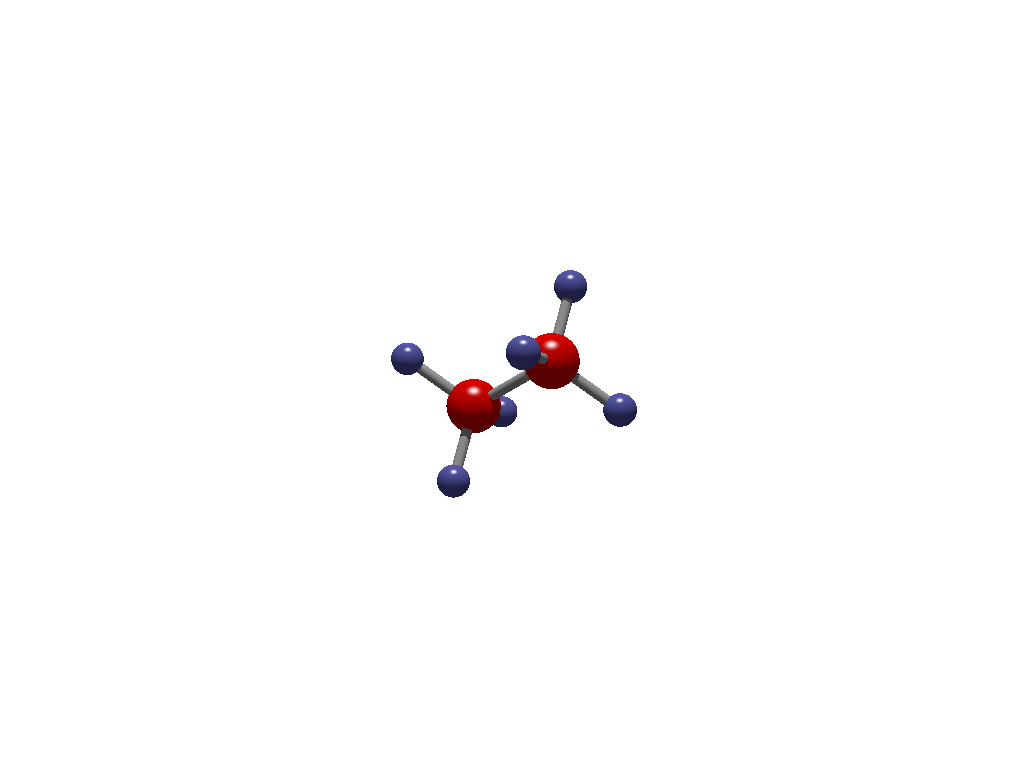
\includegraphics[height=100mm]{kadai_1.png}
\caption{課題1の画像}
\end{figure}

\clearpage

\section{課題2}
鉛筆は、芯と表面のテクスチャーと、本体のテクスチャーを引数とするマクロとして定義する。
そして鉛筆の本体のもととなるあオブジェクトを六角形プリズムとして作成し,
図4の表面Aは、プリズムとそれを僅かに縮小したものとの差として作成する。同図の木の部分Bは、プリズムを僅かに縮小したものと芯の円筒の差として作成し,また同図の芯Cは円筒として作成する。
図4のA,B,Cを最終的に結合で一つのオブジェクトにまとめて、本体を作成する。
図5の本体Dと先端Eの結合して、鉛筆Fにまとめ,先端Bは、本体と適度な大きさの円錐の交差として作成する。
鉛筆のオブジェクトはマクロによって生成し、座標変換によって配置する。

\begin{lstlisting}[style=pov,mathescape=true,caption={課題2のソースコード}, label={src:example}]

#declare N = 6;
#declare Height = 50;
#declare Default_Color = color rgb <0.5, 0.5, 0.5>;
#declare Purple = color <1, 0.0, 1>;

#declare paper = object{
    box{
        <0, 0, 0>, <1, 1, 0.01>
    }
    pigment{image_map{png "paper.png" map_type 0}}
    rotate <90, 0, 0>
    scale <100, 0.05, 141.4>
    translate <-50, 0.001, -50>
};

#declare mainbody_parts_1 =
prism{
    linear_spline
    0,Height
    N + 1
    #for(i,0,N)
    PtoR(1,360/N*i)
    #end
};

#declare mainbody_parts_2 =
cylinder{
    <0,0,0>,<0,Height,0>,0.3
    texture{
        pigment{Default_Color}
    }
};


#macro mainbody(lead_texture, surface_texture, body_texture)
    union{
        difference {
            object{mainbody_parts_1}
            object{mainbody_parts_1 scale <0.99, 1.01, 0.99>}
            texture{surface_texture}
        }
        difference {
            object{mainbody_parts_1 scale <0.99, 0.99, 0.99>}
            object{mainbody_parts_2}
            texture{body_texture}
        }
        object{mainbody_parts_2 texture{lead_texture}}
    }
#end

#macro pencil(lead_texture, surface_texture, body_texture)
    union{
        mainbody(lead_texture, surface_texture, body_texture)
        intersection{
            object{mainbody(lead_texture, surface_texture, body_texture) translate <0, Height, 0>}
            cone{<0,Height,0>,2.0,<0,Height + 10.0,0>,0}
            cutaway_textures
        }
    }
    translate(<0, -(Height + 10), 0>)
    scale <1.5, 1.5, 1.5>
#end


\end{lstlisting}

\begin{figure}[h]
\centering
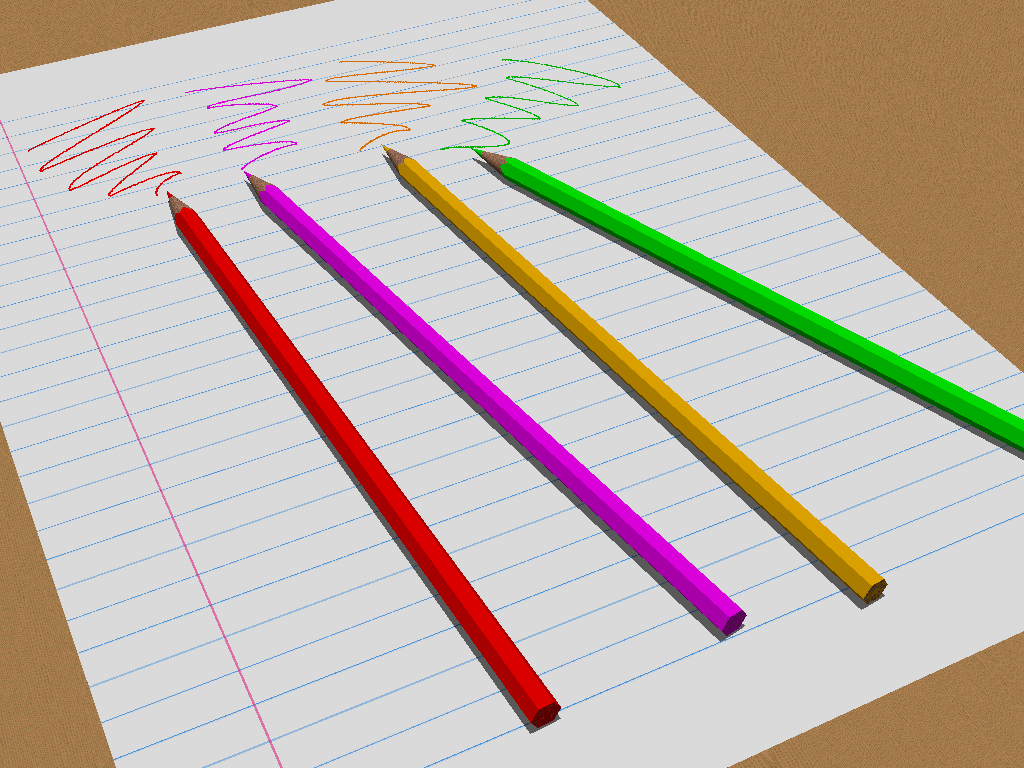
\includegraphics[height=100mm]{kadai_2.png}
\caption{課題2の画像}
\end{figure}

\clearpage

\section{課題3}
サイコロは、目の材質と本体の材質を引数としたマクロとして作成する。
本体は、立方体と球体の交差として作成する。
目を作るためのオブジェクトは球体を配置して結合で一つのオブジェクトにまとめることで作成する。目のオブジェクトは、一、二、四、六を作成し、これらを組み合わせることで三、五を作成する。
また,調整がしやすいように、ソースコードにおいて一箇所の値を変更することですべての目の大きさまたは間隔が変わるように実装する。
無限平面を用い、マクロで生成したサイコロオブジェクトに適切な座標変換を施すことで配置を行う.
\begin{lstlisting}[style=pov,mathescape=true,caption={課題3のソースコード}, label={src:example}]

#declare roll_radius = 0.1;
#declare roll_space = 0.25;

#macro roll(xpos, ypos, zpos)
object{
    sphere{<0,0,0>, roll_radius}
    translate <xpos, ypos, zpos>
}
#end

#declare roll_one =
object{
    roll(0, 0, 0)
};

#declare roll_two =
union{
    roll(-roll_space, 0, -roll_space)
    roll( roll_space, 0,  roll_space)
};

#declare roll_three =
union{
    object{roll_one}
    object{roll_two}
};

#declare roll_four =
union{
    roll(-roll_space, 0, -roll_space)
    roll(-roll_space, 0,  roll_space)
    roll(+roll_space, 0, -roll_space)
    roll(+roll_space, 0,  roll_space)
};

#declare roll_five =
union{
    object{roll_one}
    object{roll_four}
};

#declare roll_six =
union{
    roll(-roll_space, 0, 0 - roll_space)
    roll(-roll_space, 0, 0             )
    roll(-roll_space, 0, 0 + roll_space)
    roll(+roll_space, 0, 0 - roll_space)
    roll(+roll_space, 0, 0             )
    roll(+roll_space, 0, 0 + roll_space)
};

#declare roll_number=array[6]{roll_one, roll_two, roll_three, roll_four, roll_five, roll_six};

#macro body()
    object{
        intersection{
            box{<0,0,0>,<1, 1, 1>}
            sphere{<0.5, 0.5, 0.5>, 0.77}
        }
        translate <-0.5, -0.5, -0.5>
    }
#end

#macro dice(body_material, roll_material)
    difference{
        object{object{body()} material{body_material}}
        object{object{roll_number[0]} material{roll_material}                  translate <0.0, 0.5, 0.0>}
        object{object{roll_number[1]} material{roll_material} rotate<0, 0, 90> translate <0.5, 0.0, 0.0>}
        object{object{roll_number[2]} material{roll_material} rotate<90, 0, 0> translate <0.0, 0.0, 0.5>}
        object{object{roll_number[3]} material{roll_material} rotate<90, 0, 0> translate <0.0, 0.0, -0.5>}
        object{object{roll_number[4]} material{roll_material} rotate<0, 0, 90> translate <-0.5, 0.0, 0.0>}
        object{object{roll_number[5]} material{roll_material}                  translate <0.0, -0.5, 0.0>}
    }
#end
\end{lstlisting}

\begin{figure}[h]
\centering
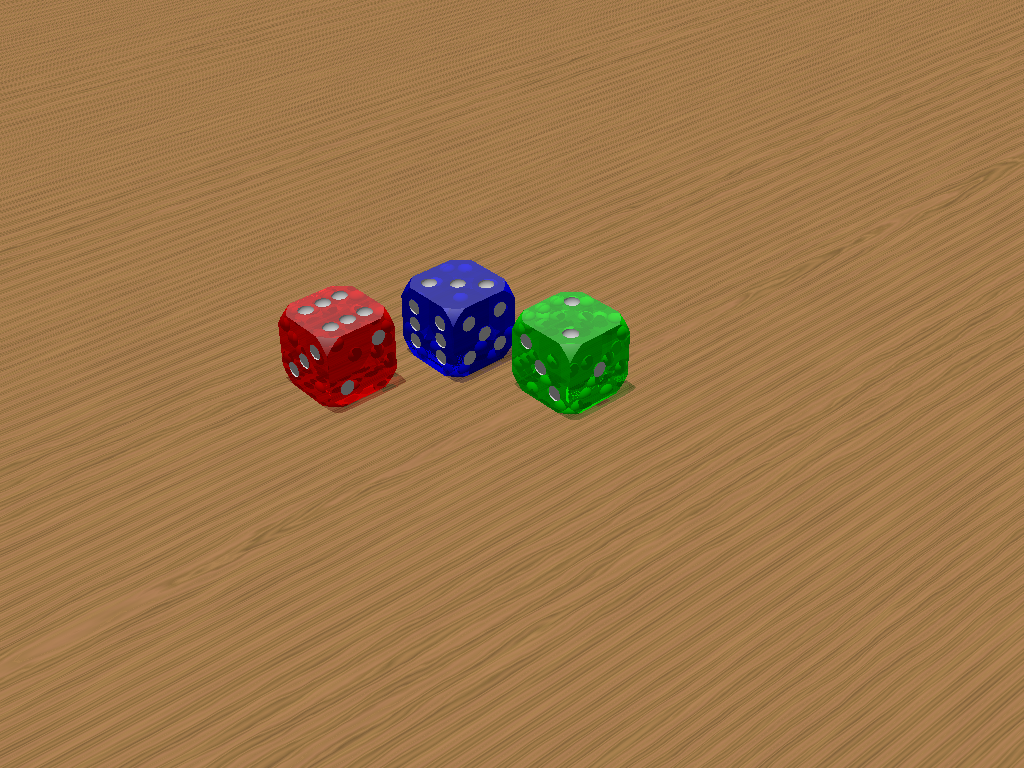
\includegraphics[height=100mm]{kadai_3.png}
\caption{課題3の画像}
\end{figure}

\clearpage

\section{課題4}
瓶のテンプレート画像を取り込んで、輪郭をBezier曲線でなぞり,瓶を回転体として作成する。
グラスも同様に、輪郭をBezier曲線で表し、回転体として作成する。
瓶のラベルは、瓶の本体より直径が僅かに大きく、適度な高さの円
筒に画像を貼り付けて、瓶と結合して一つのオブジェクトにまと
める。

\begin{lstlisting}[style=pov,mathescape=true,caption={課題4のソースコード}, label={src:example}]

camera{
    location <0.5, 1.0, -5> // カメラの位置
    look_at <0.5, 1.2, 0> // 注視点の位置
    angle 60 // 視角
}
// 光源
light_source{
    <10, 100, -100> // 光源の位置
    color White // 光源の色
}


union{
    lathe{
        bezier_spline
        BottleN,
        #for(i, 0, BottleN-1)
            BottleBP[i]
        #end

        texture {
            pigment { Col_Glass_Winebottle }
            finish{ F_Glass1 }
        }
        interior { ior 1.5 }
    }

    difference{
        cylinder{<0, 0, 0>, <0, 1, 0>, 0.42}
        cylinder{<0, 0, 0>, <0, 1.2, 0>, 0.41}
        pigment{image_map { png "wine_label.png" map_type 2 } }
        translate <0, 0.2, 0>
    }
    
    rotate <0, 150, 0>
}

union{
    lathe{
        bezier_spline
        GlassN,
        #for(i, 0, GlassN-1)
            GlassBP[i]
        #end

        material{ M_Glass3 }
    }

    
    rotate <0, 90, 0>
    translate <3, 0.0, 0>
    scale <0.4, 0.7, 0.4>
}


object{
    plane{ y, 0 rotate 2*x }
    texture{T_Grnt23}
}

sky_sphere{ S_Cloud1 }


background{color White}
\end{lstlisting}


\begin{figure}[h]
\centering
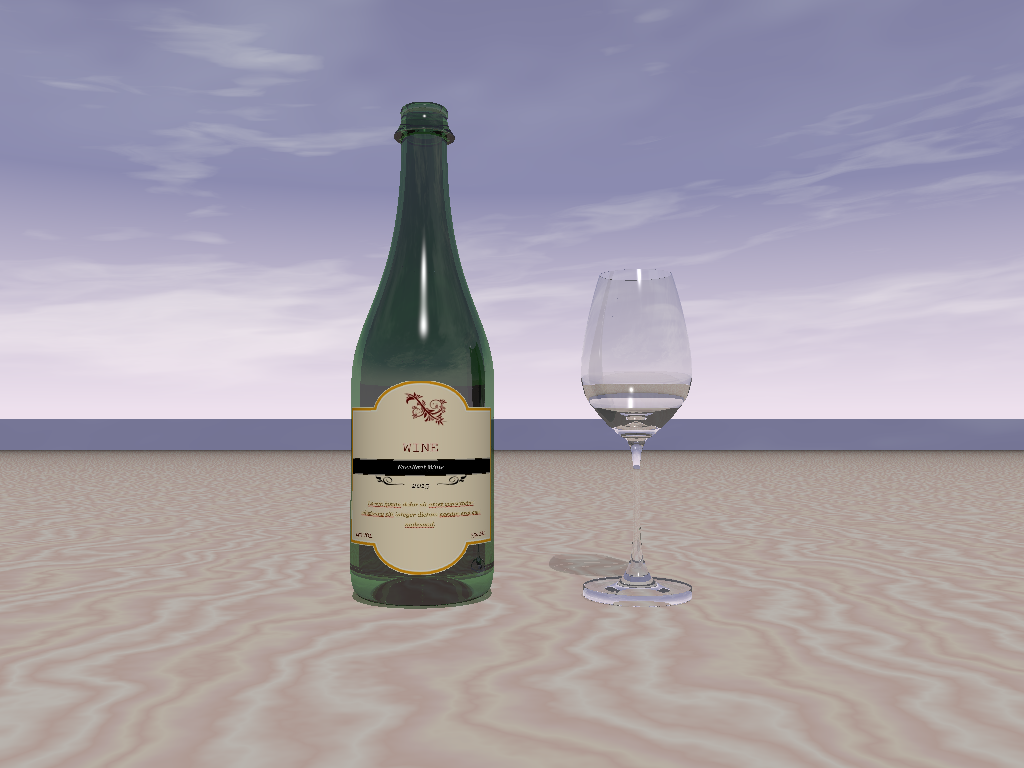
\includegraphics[height=100mm]{kadai_4.png}
\caption{課題4の画像}
\end{figure}

\clearpage

\section{考察}
POV-Rayを用いることでコンピュータグラフィックスの仕組みを理解し、シーン記述言語POV-Rayを制作に応用して使うことが出来た.C言語のようなソースコードの書式なので,非常に簡単に記述することができ,誰でも容易に幅広い環境でレイトレーシングに対応したコンピュータ・グラフィックスを生成することが可能なので,コンピュータ・グラフィックスを扱うときには活用すべきソフトウェアだと感じた.また,マクロ機能などを用いることにより簡単に部品の再利用が可能であり,複雑な図形や処理を容易に実行することができるので,シミュレータとしての利用も可能であるという点から,使い方によっては画像だけではなく動画の生成も行うことができる.コードで記述することから,3Dモデリングソフトでは手間のかかる計算による処理なども容易であり,状況によってはCADや3Dモデリングソフトよりも優れているためケースバイケースによって使い分けていきたい.
\end{document}
